\documentclass[conference]{IEEEtran}
\IEEEoverridecommandlockouts
% The preceding line is only needed to identify funding in the first footnote. If that is unneeded, please comment it out.
\usepackage{cite}
\usepackage{amsmath,amssymb,amsfonts}
\usepackage{algorithmic}
\usepackage{graphicx}
\usepackage{textcomp}
\usepackage{xcolor}
\usepackage{url}
\usepackage{tikz}
\usetikzlibrary{arrows.meta, backgrounds, calc, fit, positioning,
                shadows.blur, shapes.geometric, shapes.misc}

% ── Colour palette ─────────────────────────────────────────────
\definecolor{inputbg} {RGB}{232,240,254}
\definecolor{inputbd} {RGB}{160,190,240}
\definecolor{procbg}  {RGB}{220,238,255}
\definecolor{procbd}  {RGB}{130,180,220}
\definecolor{outbg}   {RGB}{230,249,238}
\definecolor{outbd}   {RGB}{100,190,140}
\definecolor{boxbg}   {RGB}{250,252,255}
\definecolor{boxbd}   {RGB}{150,185,225}
\definecolor{parentbg}{RGB}{235,244,255}
\definecolor{parentbd}{RGB}{80,130,200}
\definecolor{synthbg} {RGB}{248,240,255}
\definecolor{synthbd} {RGB}{148,100,210}
\definecolor{agentbd} {RGB}{110,165,220}
\definecolor{arrowcol}{RGB}{70,120,190}
\definecolor{loopcol} {RGB}{220,140,20}
\definecolor{revcolor}{RGB}{190,60,50}
\definecolor{passgreen}{RGB}{60,160,100}
\definecolor{outarrow} {RGB}{50,150,90}

\usepackage{graphics}

\usepackage{caption} 
\captionsetup[table]{skip=10pt}
\usepackage{tabularx}
\usepackage{float}
\usepackage{flushend}

%\usepackage{subfig}
\usepackage{epsfig}
\usepackage{subcaption}
\usepackage{calc}
\usepackage{amstext}
\usepackage{multicol}
\usepackage{pslatex}
\usepackage{algorithm2e}
\usepackage{comment}
\usepackage{dirtytalk}

\def\BibTeX{{\rm B\kern-.05em{\sc i\kern-.025em b}\kern-.08em
    T\kern-.1667em\lower.7ex\hbox{E}\kern-.125emX}}
\begin{document}

\title{An Open-source LLM-Assisted System for IT/SRE Triage }

\makeatletter
\newcommand{\linebreakand}{%
  \end{@IEEEauthorhalign}
  \hfill\mbox{}\par
  \mbox{}\hfill\begin{@IEEEauthorhalign}
}
\makeatother



\author{
\IEEEauthorblockN{Student}
\IEEEauthorblockA{\textit{Khoury College of Computer Sciences} \\
\textit{Northeastern University}\\
Vancouver, Canada \\
pandya.kal@northeastern.edu}
%\hspace{11.5cm}
\and

\IEEEauthorblockN{Dawood Sajjadi}
\IEEEauthorblockA{\textit{TBC} \\
\textit{}\\
 \\
}
\and
\IEEEauthorblockN{Maryam Tanha}
\IEEEauthorblockA{\textit{Khoury College of Computer Sciences} \\
\textit{Northeastern University}\\
Vancouver, Canada \\
m.tanha@northeastern.edu}
}


\maketitle
\begin{abstract}

\end{abstract}

\begin{IEEEkeywords}

\end{IEEEkeywords}
\section{Introduction}
A production incident in a cloud-native microservice architecture puts SRE and DevOps teams
under immediate pressure: they must \texttt{SSH} into multiple hosts, sift through logs, and
reconcile metrics from different monitoring systems, often in parallel, under time constraints,
and without a clear picture of what is failing~\cite{zhang2025aiops_survey, chen2024rcacopilot}.
LLMs have begun to change this picture, but not by replacing the toolchain. Survey evidence
makes clear that models must be coupled with existing systems to stay effective, not substituted
for them~\cite{zhang2025aiops_survey, szandala2025aiops_reliability}. One finding in particular
shapes our architecture: LLMs reason well about generic failure patterns but consistently fail
at \emph{topological reasoning}: they cannot trace a fault through a specific service call chain
unless the dependency graph is given to them explicitly~\cite{xu2025openrca}.

We address this with an open-source, hierarchical multi-agent framework that grounds LLM
reasoning in a YAML service topology and enforces a read-only execution model throughout the
investigation~\cite{kholkar2025safeops}. Log ingestion is handled by local ``thin sidecar''
agents that structure raw output via in-context learning before passing it upstream~\cite{xu2024divlog},
keeping evidence compact and typed rather than forwarding raw streams that would exhaust a
context window.

%\section{Background \& Motivation}


\section{Related Work}

\subsection{Multi-Agent Architectures for IT Operations}
Splitting a complex task across specialized agents consistently outperforms asking a single
model to handle everything. AgentOrchestra~\cite{zhang2025agentorchestra} formalizes this
with the TEA (Tool-Environment-Agent) protocol, where a central planner delegates to
domain-specific sub-agents; the architecture achieves 89\% on the GAIA benchmark, well above
monolithic baselines. MetaGPT~\cite{hong2024metagpt} takes a different angle: it assigns each
agent a Standard Operating Procedure modeled on human job descriptions, which constrains
output format and sharply reduces coordination errors. Both works converge on the same
conclusion: role boundaries matter as much as model capability.

Context management is where many multi-agent IT systems break down. AOI~\cite{bai2025aoi}
compresses intermediate findings before passing them to a high-level observer, retaining 92.8\%
of critical information at 72.4\% compression, while cutting mean time to recovery by 34.4\%
over the best prior baseline. Our system takes a related but stricter approach: rather than
dynamically compressing, we require each worker to emit findings in a fixed schema, which makes
downstream synthesis predictable rather than dependent on compression quality. Three IT-specific
systems also shape our design. Triangle~\cite{yu2025triangle} demonstrated over 20\% triage
accuracy improvement (reaching 91.7\% at 5-hop routing) in a production deployment serving
tens of millions of users. MasRouter~\cite{yue2025masrouter} routes queries to cheaper models
when complexity permits, cutting HumanEval inference cost by 52\%. SageCopilot~\cite{liao2025sagecopilot}
introduced a mandatory output-checking phase before delivery, a pattern we replicate in our
Evaluator Agent.

\subsection{LLM-Based Root Cause Analysis}
Production deployments reveal a pattern: raw data in, low accuracy out. RCACopilot at
Microsoft~\cite{chen2024rcacopilot} addressed this by summarizing structured diagnostic
information before passing it to the prediction model, gaining 0.077 absolute Micro-F1 points
over the unsummarized baseline. FLASH~\cite{zhang2024flash} goes further, decomposing the
full diagnostic lifecycle into four supervised states and learning from historical failure
runs; on 250 real incidents, it hit 73.9\% accuracy and brought average diagnosis time down
to 5.3 minutes against a 90-minute human mitigation baseline.

Agent separation is not just an architectural preference; it measurably shifts outcomes.
MA-RCA~\cite{fu2026marca} splits retrieval and validation into distinct agents and reports
95.8\% accuracy on the Nezha cloud-native dataset, a result the authors attribute directly
to eliminating context-switching between hypothesis generation and evidence checking.
D-Bot~\cite{zhou2023dbot} applies Tree-of-Thought reasoning to database anomalies, which
forces the planner to branch on intermediate findings rather than commit to a flat task list
upfront. Both designs directly inform how our Parent Agent re-evaluates its plan after each
worker cycle.

Not every scenario suits the same approach. Hy-LIFT~\cite{salman2025hylift} shows that for
5G/6G networks, rule-based labeling handles known fault classes well; the LLM layer is reserved
for novel or ambiguous cases, reaching a macro-F1 of roughly 89--90\%. At the other end,
the AIOps-for-Reliability study~\cite{szandala2025aiops_reliability} finds that zero-shot LLMs
misclassify benign traffic spikes as security incidents at a disturbing rate. This negative
bias prompted us to add an independent Evaluator Agent whose sole job is to challenge
the Parent Agent's conclusion before it is reported.

\subsection{Specialist Agent Design}
Ashraf and Talavera~\cite{ashraf2025autonomous} make the case empirically: specialist
multi-agent setups beat single ``super-agent'' generalists because context-switching between
domains degrades reasoning quality. We take this seriously in our worker layer, which comprises
seven narrow agents (Network, Memory, Log, Database, Cache, OS, and Application) rather than
one general-purpose investigator. The tradeoff is deliberate. A Redis-focused agent whose
system prompt encodes eviction policy, replication lag thresholds, and expected key-space
behavior will consistently outperform a model that knows ``a little about everything,'' and
in an on-call scenario, that consistency is what matters.

\subsection{Log Analysis and Preprocessing}
Dumping raw infrastructure logs into an LLM context is a well-documented failure mode: token
budgets overflow, important lines get truncated, and the model cannot distinguish noise from
signal. DivLog~\cite{xu2024divlog} addresses template extraction specifically by sampling a
maximally diverse set of log candidates offline and using them as in-context
examples at inference time. Across 16 LogPAI benchmarks it achieves 98.1\% parsing accuracy,
which makes structured templates a reliable input rather than an aspiration. Our ``thin
sidecar'' workers adopt the same principle: parse locally, emit a typed summary, and never
forward raw streams upstream.

\subsection{Agent Communication, Security, and Resilience}
How agents communicate is as consequential as what they compute. LACP~\cite{li2025lacp}
proposes a three-layer, telecom-inspired Plan-Act-Observe handshake with cryptographic
signing, adding only 0.03\,ms of overhead while making silent failures detectable. Huang
et al.~\cite{huang2024resilience} inject faulty agents into three topology types and measure
the damage: hierarchical systems lose only 5.5\% accuracy; flat topologies, lacking clear
authority, reach decision paralysis at 10.5\%; linear chains, where each hop re-transmits
errors, degrade by 23.7\%. Our workers are therefore firewalled from each other; all
findings route through the Parent Agent, which is the only entity allowed to synthesize or
escalate.

On the security side, Kholkar and Ahuja~\cite{kholkar2025safeops} demonstrate a
``policy-as-prompt'' pattern that encodes governance rules into runtime classifiers; their
least-privilege framing is the direct academic grounding for our read-only execution default.
Looking ahead to Phase~2, the AWS MCP architecture~\cite{aws2025mcp_sre} shows how Model
Context Protocol servers allow agents to discover tools dynamically without bespoke API
wrappers, offering a practical path to extending our worker roster without modifying the core
orchestration graph.


\section{Methodology}

% ─────────────────────────────────────────────────────────────
%  ARCHITECTURE FIGURE
% ─────────────────────────────────────────────────────────────
\begin{figure*}[t]
\centering
\makebox[\textwidth][c]{%
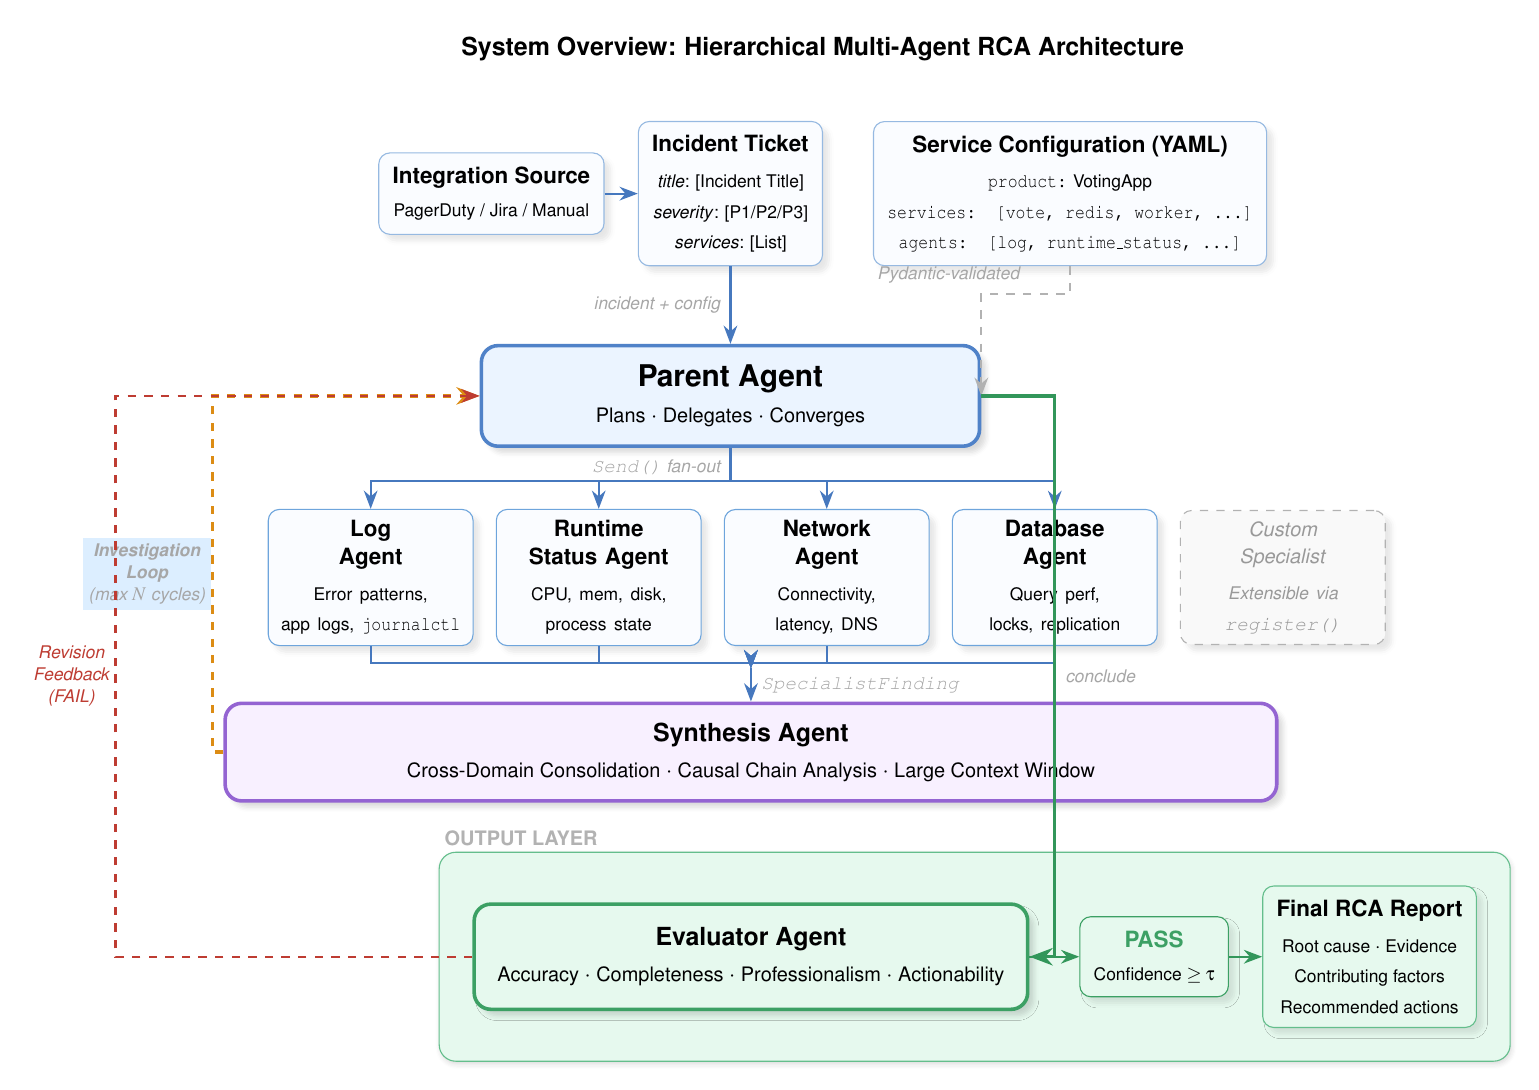
\begin{tikzpicture}[
  font=\small\sffamily,
  >=Stealth,
  layer/.style  = {draw, rounded corners=6pt, inner sep=12pt,
                   blur shadow={shadow blur steps=5, shadow xshift=0.5pt,
                                shadow yshift=-1pt, shadow opacity=15}},
  box/.style    = {draw=boxbd, fill=boxbg, rounded corners=4pt,
                   inner sep=5pt, minimum height=22pt, align=center,
                   blur shadow={shadow blur steps=3, shadow opacity=10}},
  agent/.style  = {draw=agentbd, fill=boxbg, rounded corners=4pt,
                   inner sep=4pt, minimum width=70pt, minimum height=38pt,
                   align=center, text width=66pt,
                   blur shadow={shadow blur steps=3, shadow opacity=10}},
  parent/.style = {draw=parentbd, fill=parentbg, rounded corners=6pt,
                   inner sep=7pt, minimum width=180pt, minimum height=36pt,
                   align=center, line width=1.3pt,
                   blur shadow={shadow blur steps=4, shadow opacity=15}},
  synth/.style  = {draw=synthbd, fill=synthbg, rounded corners=6pt,
                   inner sep=7pt, minimum width=380pt, minimum height=32pt,
                   align=center, line width=1.3pt,
                   blur shadow={shadow blur steps=4, shadow opacity=15}},
  evalbox/.style= {draw=passgreen, fill=outbg, rounded corners=6pt,
                   inner sep=7pt, minimum width=200pt, minimum height=38pt,
                   align=center, line width=1.3pt,
                   blur shadow={shadow blur steps=4, shadow opacity=15}},
  arr/.style    = {->, thick, color=arrowcol},
  arrgr/.style  = {->, thick, color=outarrow},
  looparr/.style= {->, very thick, color=loopcol, dashed},
  revarr/.style = {->, thick, color=revcolor, dashed},
  sublabel/.style = {font=\fontsize{7}{8}\selectfont\sffamily\itshape,
                     color=gray!70},
]

% ── INPUT LAYER ────────────────────────────────────────────────
\node[box] (src) {
  \textbf{Integration Source}\\[1pt]
  {\fontsize{7}{8}\selectfont PagerDuty / Jira / Manual}
};

\node[box, right=12pt of src] (ticket) {
  \textbf{Incident Ticket}\\[2pt]
  {\fontsize{7}{8}\selectfont\textit{title}: [Incident Title]}\\
  {\fontsize{7}{8}\selectfont\textit{severity}: [P1/P2/P3]}\\
  {\fontsize{7}{8}\selectfont\textit{services}: [List]}
};

\node[box, right=18pt of ticket] (yaml) {
  \textbf{Service Configuration (YAML)}\\[2pt]
  {\fontsize{7}{8}\selectfont\texttt{product:} VotingApp}\\
  {\fontsize{7}{8}\selectfont\texttt{services: [vote, redis, worker, \ldots]}}\\
  {\fontsize{7}{8}\selectfont\texttt{agents: [log, runtime\_status, \ldots]}}
};

\begin{pgfonlayer}{background}
  \node[layer, draw=inputbd, fill=inputbg,
        fit=(src)(ticket)(yaml),
        label={[anchor=south west, inner sep=2pt, font=\fontsize{8}{9}\selectfont\sffamily\bfseries,
                text=gray!60] north west:INPUT LAYER}] (inputlayer) {};
\end{pgfonlayer}

\draw[arr] (src.east) -- (ticket.west);

% ── PROCESSING LAYER ───────────────────────────────────────────
\node[parent, below=28pt of ticket] (parent) {
  \textbf{\large Parent Agent}\\[2pt]
  {\fontsize{8}{9}\selectfont Plans $\cdot$ Delegates $\cdot$ Converges}
};

\node[agent, below=22pt of parent, xshift=-130pt] (logagent) {
  \textbf{Log}\\[-1pt]\textbf{Agent}\\[2pt]
  {\fontsize{7}{8}\selectfont Error patterns,}\\
  {\fontsize{7}{8}\selectfont app logs, \texttt{journalctl}}
};

\node[agent, right=8pt of logagent] (rtagent) {
  \textbf{Runtime}\\[-1pt]\textbf{Status Agent}\\[2pt]
  {\fontsize{7}{8}\selectfont CPU, mem, disk,}\\
  {\fontsize{7}{8}\selectfont process state}
};

\node[agent, right=8pt of rtagent] (net) {
  \textbf{Network}\\[-1pt]\textbf{Agent}\\[2pt]
  {\fontsize{7}{8}\selectfont Connectivity,}\\
  {\fontsize{7}{8}\selectfont latency, DNS}
};

\node[agent, right=8pt of net] (db) {
  \textbf{Database}\\[-1pt]\textbf{Agent}\\[2pt]
  {\fontsize{7}{8}\selectfont Query perf,}\\
  {\fontsize{7}{8}\selectfont locks, replication}
};

\node[agent, right=8pt of db, dashed, draw=gray!60, text=gray!80, fill=gray!5] (ext) {
  {\fontsize{8}{9}\selectfont\textit{Custom}}\\[-1pt]
  {\fontsize{8}{9}\selectfont\textit{Specialist}}\\[2pt]
  {\fontsize{7}{8}\selectfont\textit{Extensible via}}\\
  {\fontsize{7}{8}\selectfont\textit{\texttt{register()}}}
};

\node[synth, below=20pt of rtagent, xshift=55pt] (synth) {
  \textbf{\normalsize Synthesis Agent}\\[2pt]
  {\fontsize{8}{9}\selectfont
   Cross-Domain Consolidation $\cdot$
   Causal Chain Analysis $\cdot$
   Large Context Window}
};

\begin{pgfonlayer}{background}
  \node[layer, draw=procbd, fill=procbg,
        fit=(parent)(logagent)(rtagent)(net)(db)(ext)(synth),
        label={[anchor=south west, inner sep=2pt, font=\fontsize{8}{9}\selectfont\sffamily\bfseries,
                text=gray!60] north west:PROCESSING LAYER}] (proclayer) {};
\end{pgfonlayer}

% ── OUTPUT LAYER ───────────────────────────────────────────────
\node[evalbox, below=36pt of synth] (eval) {
  \textbf{\normalsize Evaluator Agent}\\[2pt]
  {\fontsize{8}{9}\selectfont
   Accuracy $\cdot$ Completeness $\cdot$
   Professionalism $\cdot$ Actionability}
};

\node[box, right=18pt of eval, draw=passgreen, fill=outbg] (pass) {
  {\color{passgreen}\textbf{PASS}}\\[1pt]
  {\fontsize{7}{8}\selectfont Confidence $\geq\tau$}
};

\node[box, right=12pt of pass, draw=outbd, fill=outbg] (report) {
  \textbf{Final RCA Report}\\[2pt]
  {\fontsize{7}{8}\selectfont Root cause $\cdot$ Evidence}\\
  {\fontsize{7}{8}\selectfont Contributing factors}\\
  {\fontsize{7}{8}\selectfont Recommended actions}
};

\begin{pgfonlayer}{background}
  \node[layer, draw=outbd, fill=outbg,
        fit=(eval)(pass)(report),
        label={[anchor=south west, inner sep=2pt, font=\fontsize{8}{9}\selectfont\sffamily\bfseries,
                text=gray!60] north west:OUTPUT LAYER}] (outlayer) {};
\end{pgfonlayer}

% ── ARROWS ─────────────────────────────────────────────────────

% Input → Parent
\draw[arr] (ticket.south)
    -- node[left, sublabel]{incident + config}
    (parent.north);

% YAML → Parent
\coordinate (yamldown) at ($(yaml.south) + (0,-10pt)$);
\draw[arr, dashed, color=gray!60]
    (yaml.south)
    -- (yamldown)
    -- node[above, sublabel, xshift=-28pt]{Pydantic-validated}
    (parent.east |- yamldown)
    -- (parent.east);

% Parent → Specialists (fan-out)
\coordinate (fanout) at ($(parent.south) + (0,-12pt)$);
\draw[arr] (parent.south) -- node[left, sublabel, yshift=-1pt]{\texttt{Send()} fan-out} (fanout) -| (logagent.north);
\draw[arr] (fanout) -| (rtagent.north);
\draw[arr] (fanout) -| (net.north);
\draw[arr] (fanout) -| (db.north);

% Specialists → Synthesis (fan-in)
\coordinate (fanin) at ($(synth.north) + (0,12pt)$);
\draw[arr] (logagent.south) -- ++(0,-6pt) -| (fanin);
\draw[arr] (rtagent.south)  -- ++(0,-6pt) -| (fanin);
\draw[arr] (net.south)      -- ++(0,-6pt) -| (fanin);
\draw[arr] (db.south)       -- ++(0,-6pt) -| (fanin);
\draw[arr] (fanin) -- node[right, sublabel]{\texttt{SpecialistFinding}} (synth.north);

% Synthesis → Parent (investigation loop, left side)
\coordinate (loopX) at ($(logagent.west) + (-20pt, 0)$);
\draw[looparr] (synth.west) -- (synth.west -| loopX)
    -- node[left, sublabel, align=center, fill=procbg, inner sep=2pt]{%
         \textbf{Investigation}\\
         \textbf{Loop}\\
         (max $N$ cycles)}
    (parent.west -| loopX) -- (parent.west);

% Parent → Evaluator (when concluding) — drop through gap between eval and pass
\coordinate (concludeGap) at ($(eval.east) + (9pt, 0)$);
\draw[arrgr, very thick]
    (parent.east)
    -- (parent.east -| concludeGap)
    -- node[right, sublabel]{conclude}
    (concludeGap)
    -- (eval.east);

% Evaluator → Pass → Report
\draw[arrgr] (eval.east) -- (pass.west);
\draw[arrgr] (pass.east) -- (report.west);

% Revision feedback (FAIL path)
\coordinate (failX)  at ($(logagent.west) + (-55pt, 0)$);
\draw[revarr] (eval.west) -- (eval.west -| failX)
    -- node[left,
            font=\fontsize{7}{8}\selectfont\sffamily\itshape\color{revcolor},
            align=center, fill=white, inner sep=2pt]{Revision\\Feedback\\(FAIL)}
    (parent.west -| failX) -- (parent.west);

% ── Title ──────────────────────────────────────────────────────
\node[above=6pt of inputlayer,
      font=\normalsize\sffamily\bfseries]
  {System Overview: Hierarchical Multi-Agent RCA Architecture};

\end{tikzpicture}%
}% end makebox
\caption{Multi-agent RCA architecture. The Parent Agent fans out
  investigation subtasks in parallel and iterates until the Evaluator
  Agent approves the draft report or the cycle limit is reached.
  Dashed red path: revision feedback on a failing evaluation.}
\label{fig:architecture}
\end{figure*}

% ─────────────────────────────────────────────────────────────
%  METHODOLOGY TEXT
% ─────────────────────────────────────────────────────────────

Fig.~\ref{fig:architecture} shows the full system. We built it as a
three-tier LangGraph graph: a Parent Agent that plans and decides, a
pool of Specialist Agents that gather evidence in parallel, and a
Synthesis Agent that correlates findings across domains before the
next cycle. An Evaluator Agent reviews the draft RCA report before it
is released.

\subsection{Service Configuration}

We wanted operators to describe their infrastructure once, in a format
they already understand, without writing any agent-specific code. The
result is a per-product YAML file validated by Pydantic at startup.

Each entry in the \texttt{services} block captures what a healthy
instance looks like (\texttt{expected\_behavior}), what patterns
signal trouble (\texttt{known\_failures}), and which shell commands
collect an initial evidence snapshot before the investigation begins
(\texttt{context\_commands}). An \texttt{agents} key references
separate YAML files describing each specialist, including routing
guidance (\texttt{when\_to\_use}, \texttt{do\_not\_use}) that the
Parent Agent reads verbatim when deciding whom to assign. Nothing
is hardcoded in the planner prompt; the topology is loaded at
invocation time, so adding a service means editing one file.

\subsection{Parent Agent and Planning}

The Parent Agent is the only node in the graph that can change the
investigation's direction. At each cycle it receives the incident
summary, the full YAML topology, and the accumulated
\texttt{cumulative\_history} from all prior cycles. We bind the LLM
with \texttt{tool\_choice=``any''} to ensure it always produces a
typed action rather than free text.

The LLM has exactly two choices. \texttt{create\_subtasks} emits a
list of \texttt{Subtask} objects, each specifying a target service,
container, natural-language description, a falsifiable hypothesis, and
the specialist to assign. The LangGraph router converts these into
\texttt{Send()} fan-out dispatches that run in parallel.
\texttt{write\_rca\_conclusion} closes the cycle, producing a
structured report with root cause, contributing factors, evidence
summary, and recommended actions.

We chose not to rely on the agent voluntarily concluding: once
\texttt{current\_cycle} reaches \texttt{MAX\_CYCLES} (default:~3),
the framework hard-wires \texttt{write\_rca\_conclusion} as the only
permitted tool call; the loop cannot run indefinitely.

\subsection{Specialist Agents}

A specialist is a LangChain ReAct agent with a deliberately narrow
scope. Its only tool is \texttt{run\_command}; its system prompt
encodes domain knowledge for one area (logs, runtime resources,
network connectivity, database internals, etc.) and nothing else.
We found that narrowing the prompt sharply reduced
cross-domain confusions: a log agent that also ``knows about''
Redis tends to reach for Redis commands at the wrong time.

Before the ReAct loop begins, the framework pre-runs the service's
\texttt{context\_commands} and, in Docker mode, tails the container
logs. Both are injected into the agent's opening message, giving it
a concrete evidence baseline without spending any tool-call budget.
The loop then runs until the agent emits a structured final answer or
hits \texttt{MAX\_ITERATIONS} (default:~10), at which point a
low-confidence \texttt{SpecialistFinding} is returned so the cycle
can continue rather than crash.

Commands run through one of two backends, both presenting the same
interface to the agent. \textit{Docker exec} calls
\texttt{docker exec <container> sh -c <cmd>} on the local host and
is the default for demo deployments. \textit{SSH} uses a pooled
paramiko client keyed by \texttt{(host, port, username)}, reusing
open transport sessions to avoid repeated handshake overhead in
production environments.

Adding a specialist requires no changes to the orchestration layer.
A new module calls \texttt{register()} at import time; the graph
builder wires the new node in at startup and the Parent Agent sees it
in its routing prompt the next invocation.

\subsection{Synthesis and Evaluation}

After each cycle's specialists finish, the Synthesis Agent reads the
new \texttt{SpecialistFinding} objects (tracked via a
\texttt{findings\_offset} pointer to avoid reprocessing prior cycles)
and produces a \texttt{CycleSummary}: a narrative paragraph,
\texttt{KEY\_FINDINGS} bullets, and \texttt{RECOMMENDATIONS}. We give
it no tool access deliberately; its job is cross-domain correlation,
noticing for example that a memory spike on the Redis container
explains the connection-pool exhaustion a log agent reported on the
API service. Keeping it tool-free means reasoning over the full
evidence window without branching into further data collection.
The resulting summary feeds into \texttt{cumulative\_history}, which
the Parent Agent reads at the start of every subsequent cycle.

When the Parent Agent calls \texttt{write\_rca\_conclusion}, the draft
report goes to the Evaluator Agent rather than directly to the user.
The Evaluator scores it on accuracy, completeness, professionalism,
and actionability. A passing score releases the report; a failing
score sends structured revision feedback back to the Parent Agent,
which re-enters the loop with that feedback as additional context.

\subsection{Security Model}

We treat agents as untrusted code paths. Every command, regardless of
which specialist issues it, passes through two sequential checks before
execution and before its output reaches the LLM.

The \textit{command allowlist} applies a deny-first rule: a command is
rejected the moment it matches any blocked pattern (destructive
operations such as \texttt{rm} and \texttt{chmod}; shell redirection;
code injection via \texttt{| bash}; and outbound network tools like
\texttt{curl} and \texttt{nc}). Only commands whose prefix appears on
the explicit allow-list (log readers, system status utilities, and
service CLIs like \texttt{redis-cli} and \texttt{psql}) proceed to
execution. Rejected commands return \texttt{"BLOCKED: <reason>"} so
the agent can adapt rather than hang.

The \textit{output redactor} scrubs every response before it leaves
the execution layer. It strips AWS access keys, PEM private-key
blocks, bearer tokens, credential assignments
(\texttt{api\_key=}, \texttt{password=}), email addresses, full IPv4
addresses (partially preserved for subnet context), and long base64
strings. The redactor runs on every execution path, including the
host-side \texttt{docker logs} fetch, so no raw secrets ever appear
in the LLM's context.

Both checks are non-negotiable at every node. The least-privilege
principle~\cite{kholkar2025safeops} holds across the entire system:
agents can read diagnostic state but cannot alter it, exfiltrate
credentials, or escalate beyond their assigned investigation scope.


\section{Experiments and Results}


\section{Conclusion and Future Directions}



%% The acknowledgments section is defined using the "acks" environment
%% (and NOT an unnumbered section). This ensures the proper
%% identification of the section in the article metadata, and the
%% consistent spelling of the heading.

\section*{Acknowledgment}

%%
%% The next two lines define the bibliography style to be used, and
%% the bibliography file.
\bibliographystyle{ieeetr}
\bibliography{references}

%%
%% If your work has an appendix, this is the place to put it.
%\appendix
  


\end{document}
\endinput
%%
%% End of file `sample-authordraft.tex'.
